\chapter{Descripción de los datos}
\label{capitulo 1}



Para el cálculo del régimen de caudal natural de una cuenca hidrológica es necesario contar con series temporales de 
precipitación y temperatura que reflejen las condiciones climáticas de las subcuencas así como ciertos descriptores
como área, pendiente, ...


Los datos de clima (precipitación y temperatura) fueron medidos a través de estaciones meteorológicas distribuidas de manera 
irregular a lo largo de la cuenca. Las series disponibles reflejan adecuadamente las condiciones climáticas de las zonas bajas y más pobladas,
pero la información en las zonas más altas es escasa. Los pluviómetros se encuentran a altitudes de entre
los 2000 y 3000 metros sobre el nivel del mar, mientras que el punto más alto de la cuenca se encuentra a las 6288 m.s.n.m

Con el fin de contrastar si estas series reflejan 
correctamente las variaciones del patrón de lluvias con la altura y la pendiente, 
se han analizado diversas bases de datos globales de precipitación pero el resultado no ha sido 
satisfactorio.  Por ello, se ha optado por generar las series de precipitación de manera sintéticas basándose 
en los patrones combinados de los pluviómetros y de las estaciones de aforos.



\section{Series de precipitación basadas en la interpolación de pluviómetros}
\label{seriespluv}
La cuenca del río Chambo posee una gran variación en la precipitación en un área geográfica reducida,
por este motivo los valores de precipitación recogidos por pluviómetros en las estaciones meteorológicas 
pueden no ser válidos para puntos lejanos. Es por eso que los datos correspondientes a puntos intermedios se 
completaron a partir de la base de datos de ERA5 y CHELSA.
\begin{figure}[h!]
  \begin{center}
    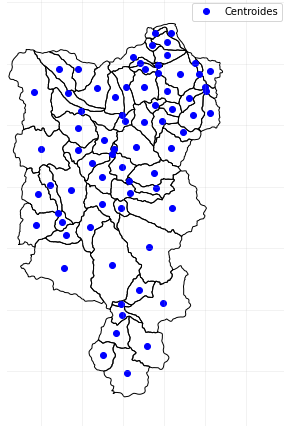
\includegraphics[height=3.in]{Figures/centroides.png}
    \caption{ Localización de los centroides de las subcuencas}
    \label{0}
  \end{center}
\end{figure}

 Una vez que los huecos han sido rellenados, se han interpolado los datos recogidos por los pluviómetros a los centroides 
 de las regiones  representadas en la figura \ref{0}. Este proceso consta de dos pasos, primero se estima si en un punto 
 determinado va a llover (estimación kriging con la librería \textit{Krige} de r) y luego se estima la magnitud de dicha 
 lluvia (Herrera et al., 2012).

 \begin{figure}[h!]
  \begin{center}
    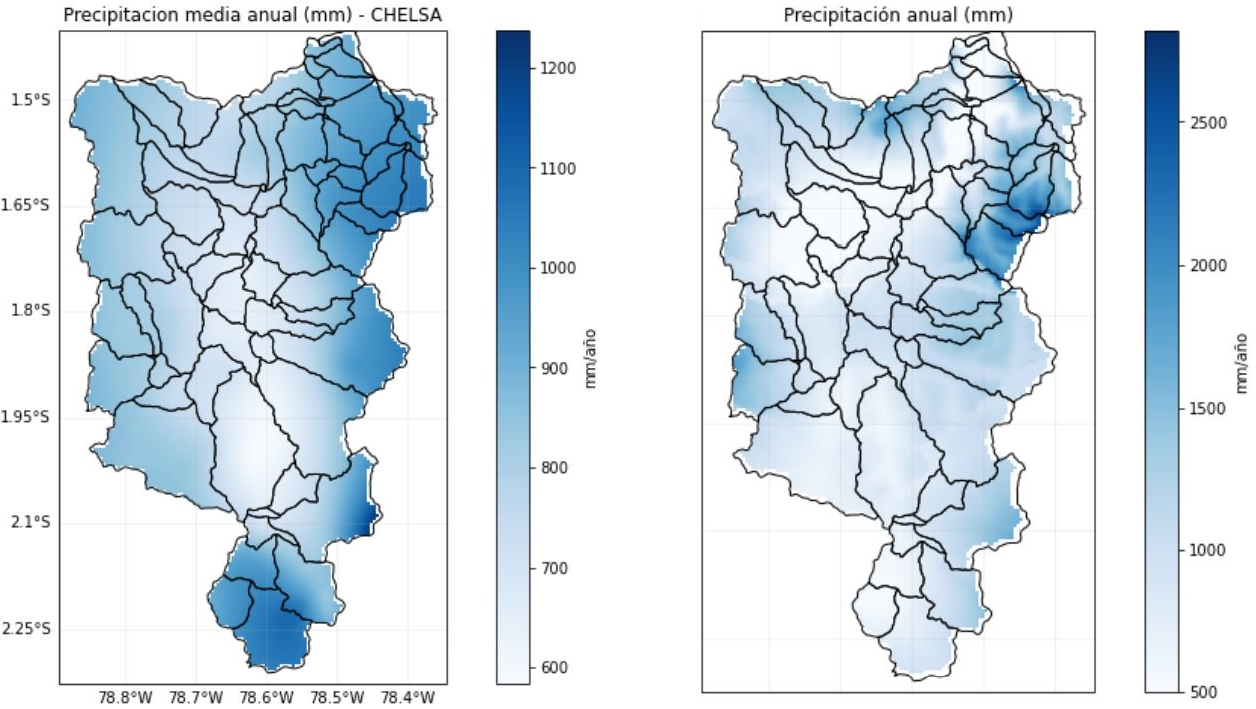
\includegraphics[height=3.in]{Figures/CHELSA_ERA5.jpg}
    \caption{ Precipitación media anual (mm/año) basada en CHELSA (panel izquierdo) y en ERA5 (panel derecho).}
    \label{1}
  \end{center}
\end{figure}


 En la figura \ref{1} se muestra a modo de ejemplo los  valores de la precipitación media anual  obtenidos mediante interpolación 
 sobre una malla regular de 100 m de lado utilizando la base de datos de ERA5 (panel derecho) y la de CHELSA (panel izquierdo).
 Si bien los resultados reflejan correctamente la fuerte variabilidad de la precipitación en un area reducida, los patrones estacionales
 así obtenidos no coinciden con los caudales y el conocimiento local. Es por eso que se ha optado por generar las series 
 de manera sintética como se describe en la siguiente sección.




\section{Generación de series sintéticas}
El modelo que genera las series de precipitación diaria consta de dos niveles, primero se generan series mensuales y
luego se generan series diarias desagregando los valores mensuales.

Para generar las series mensuales se parte del valor medio anual en la región climática y del valor medio en el 
mes más húmero.
Se han definido a su vez, tres patrones de precipitación para diferentes regiones:
1) costero, donde la precipitación máxima tiene lugar en el mes de abril, y un segundo pico inferior al de abril, en torno a octubre-noviembre.
2) amazónico, con un único pico de precipitación en junio-julio, y el mínimo en diciembre-enero y 3) mixto que es una combinación de los dos primeros. 


La precipitación media anual de cada subcuenca  se ha determinado basándose en la interpolación de los datos de 
pluviómetros con la base de datos CHELSA ya que en términos de magnitud es la más exacta.
Por otro lado el tipo de régimen así como el patrón de estacionalidad de los caudales se han determinado en información disponible
localmente  (\textcolor{codegreen}{Es así??}).

El modelo de desagregación a escala mensual asume que las precipitaciones acumuladas en cada mes siguen un comportamiento
que puede ser representado por la siguiente distribución Log-normal con una variación temporal sinusoidal y
desviación estándar $s_1$:

\begin{equation}
    P_m=exp\Bigg(N\bigg(a+b1\cdot cos\bigg(\frac{t-\phi_1}{6}\bigg)+b2\cdot cos\bigg(\frac{t-\phi_2}{12}\bigg)\bigg)\Bigg)
\end{equation}

$N(\mu,\sigma)$ es a su vez una distribución Gaussiana con media $\mu$ y desviación estándar $\sigma$. 
Los valores de las constantes $a$, $b_1$ y $b_2$ se obtienen a partir de la precipitación media y máxima, 
mientras que las fases $\phi_i$ dependen del régimen de precipitación.

\begin{figure}[h!]
    \begin{center}
      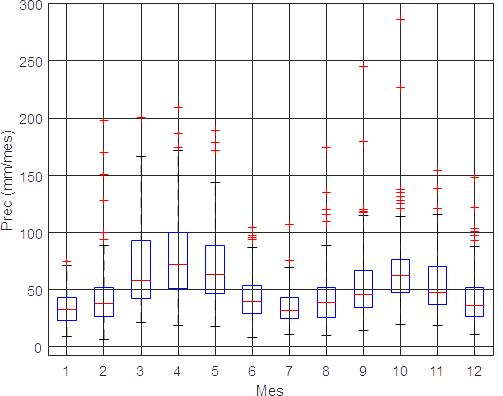
\includegraphics[height=3.in]{Figures/prec_sim.png}
      \caption{ Valores simulados de precipitaciones mensuales en la zona de Guaslán}
      \label{2}
    \end{center}
  \end{figure}


En la figura \ref{2} se muestra a modo de ejemplo una de las series generada para una cuenca con clima costero, representativa del sector más 
seco de la cuenca en la estación de Guaslán (cantón Riobamba). La línea roja representa el valor medio, la caja azul representa los valores situados entre los percentiles
 25$\%$ y 75$\%$, y las barras negras los extremos (los puntos en rojo son tratados como datos atípicos). A modo de comparación,
 en la figura \ref{3} se muestran los valores observados en la misma estación.

 \begin{figure}[h!]
    \begin{center}
      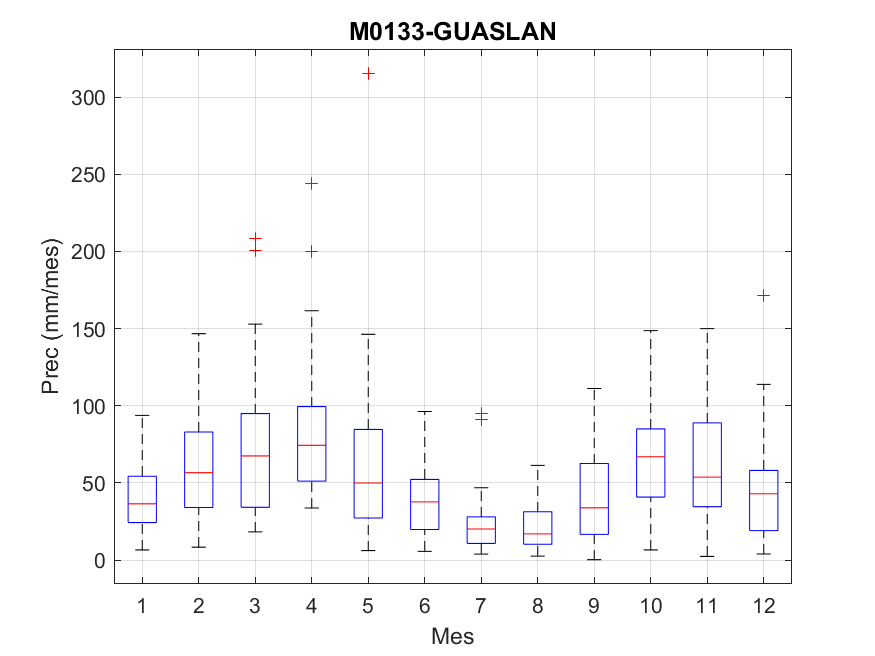
\includegraphics[height=3.in]{Figures/prec_obs.png}
      \caption{ Valores observados de precipitaciones mensuales en la zona de Guaslán}
      \label{3}
    \end{center}
  \end{figure}

  \begin{figure}[h!]
    \begin{center}
      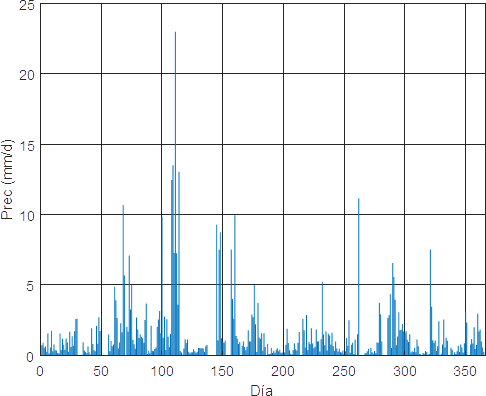
\includegraphics[height=3.in]{Figures/prec_sint.png}
      \caption{ Un año de valores de precipitación diaria simulada en la zona de Guaslán}
      \label{3}
    \end{center}
  \end{figure}


El modelo para crear las series diarias usa el método de cascadas aleatorias multiplicativas (Molnar y Burlando (2005)) para 
desagregar las series mensuales. El modelo consta de dos parámetros: denominados $sig2$ y $beta$
que determinan la variabilidad e intermitencia de la lluvia (proporción media de días sin lluvia) y se usan para 
ajustar el modelo, con los valores observados en las series de precipitación disponibles.
La Figura  muestra la serie obtenida para la estación de Guaslán.

\subsubsection{Comportamiento del régimen de precipitación}
\label{regimenes_prec}
Con el fin de poder realizar un estudio completo de cómo es el comportamiento del régimen de precipitaciones, 
se seleccionaron 35 estaciones  meteorológicas que abarcan de manera uniforme el area de la cuenca de Chambo y sus alrededores.
Se han identificado principalmente dos regímenes diferentes, un régimen bimodal en el oeste (dos períodos secos y dos de lluvias al año) 
y el régimen monomodal (un período seco y uno de lluvias) en el este, con una franja que contiene un régimen mixto en 
las zonas centrales de la cuenca.




% En la figure \ref{4}, se muestran a modo de ejemplo las series de precipitación generadas para tres diferentes subcuencas 
% localizadas en diferentes puntos durante los años 2000, 2010 y 2019. Se puede observar las diferentes estacionalidades,
% en la localizada más al norte un régimen costero, en la localizada más al sur un régimen amazónico, mientras que la cuenca 
% localizada más al oeste presenta un clima más árido. 


\begin{figure}[h!]
  \begin{center}
    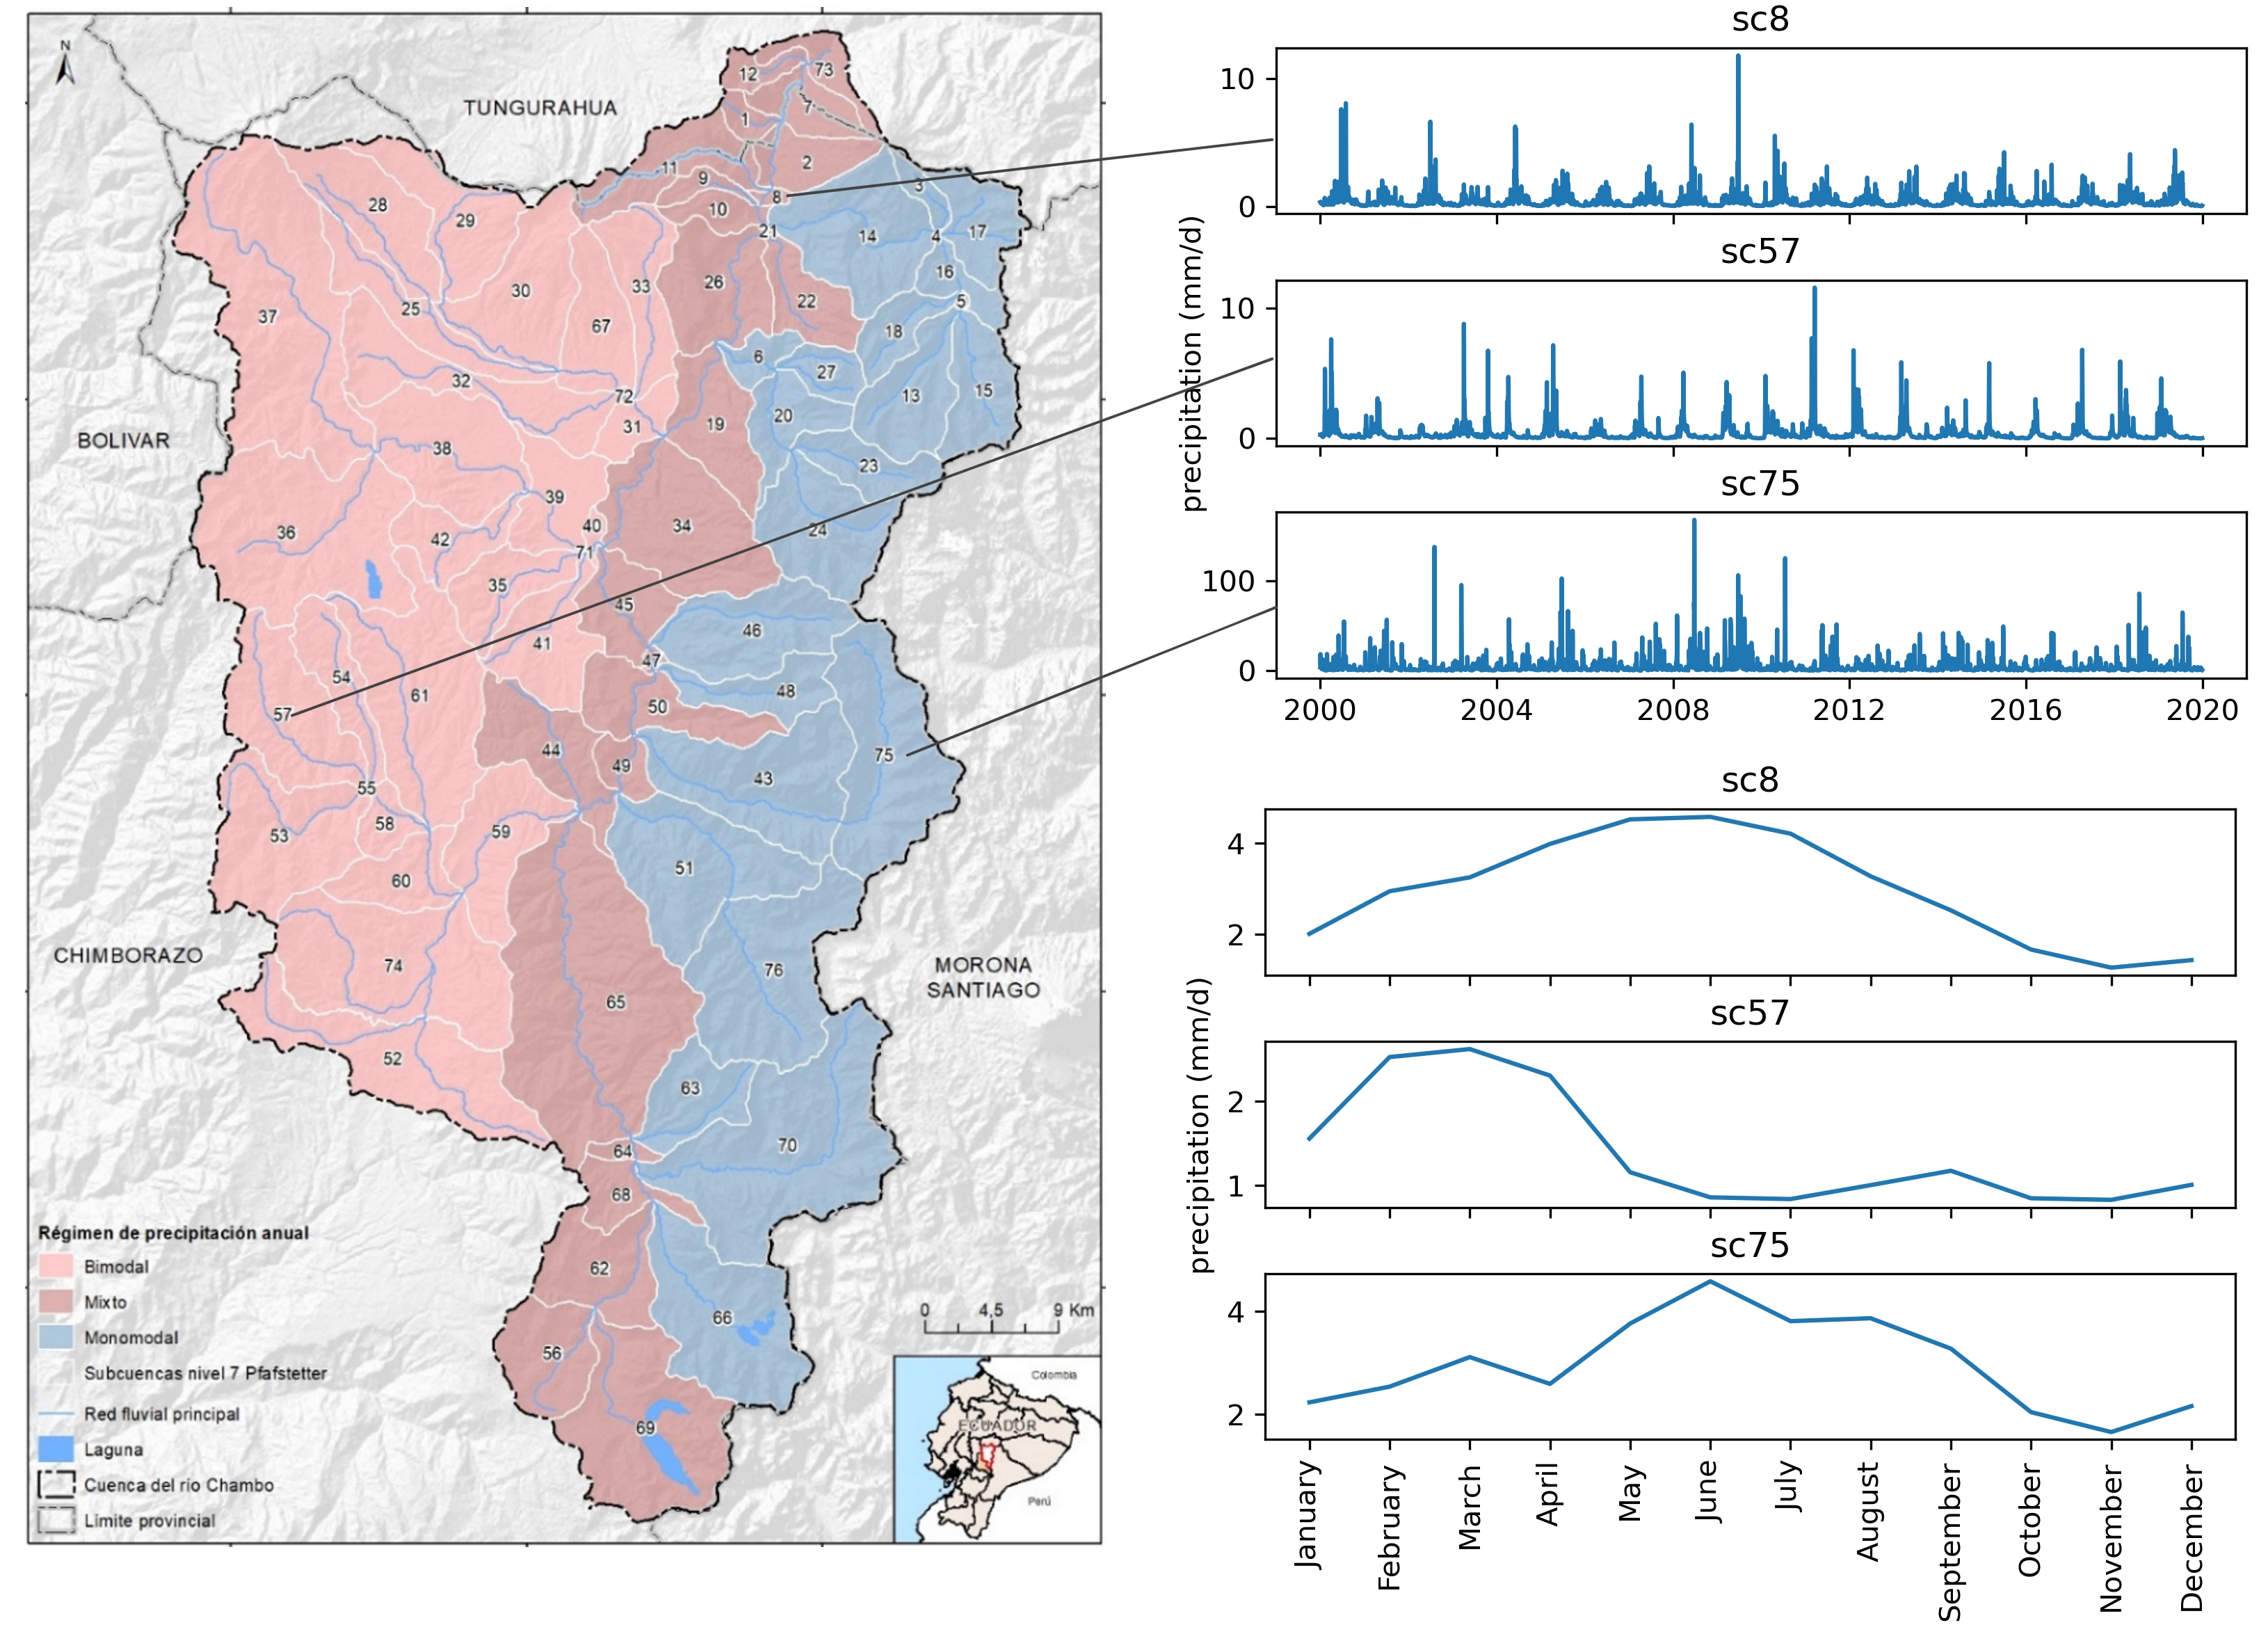
\includegraphics[height=4.in]{Figures/cuenca_con_subcuencas_prec.png}
    \caption{ Series de precipitación para diferentes regiones de la cuenca Chambo. En el panel superior derecho se muestrala serie 
    de precipitación correspondiente al año 2019 y en el panel inferior los valores medios mensuales desde el año 2000 hasta el año 2020.}
    \label{4}
  \end{center}
\end{figure}




\section{Temperatura}
\label{tempint}
Para la generación de las series de temperatura se utilizado datos de 10 termómetros situados en el entorno del área de estudio.
Estos datos han sido sometidos al siguiente proceso de curado:

\begin{enumerate}
  \item Se ha definido una frontera para detectar outliers o datos atípicos siguiendo el siguiente criterio:
  \begin{equation}
    si~X_i>5\cdot\sigma^2_n~es~un~utlier,~donde~\sigma^2_n=\frac{1}{n}\cdot\sum^n_{i=1}\bigg(X_i-\bar{X}\bigg)^2
  \end{equation}
  \item Eliminación de datos consecutivos repetidos. La persistencia del mismo valor puede sugerir errores 
  de transcripción o problemas en el caso de instrumentos con registro electrónico de datos, por ejemplo, en estaciones meteorológicas automáticas (Estévez et al., 2011).
\end{enumerate}

De manera similar a cómo se procedió con las series de precipitación en la sección \ref{seriespluv}, se han completados
los datos faltantes y huecos espaciales utilizando los datos de ERA5. En la figura ... se muestran las series de temperaturas 
máximas y mínimas para diferentes puntos de la cuenca.
\textcolor{codegreen}{armar gráfica}
\textcolor{codegreen}{explicar las gráficas}


% \subsection{Series temporales de temperatura}
% Las temperaturas diarias por subcuencas se obtiene de la información de los rásteres (\textcolor{codegreen}{SI??}),
% las temperaturas máximas y mínimas diarias, $T_{max}$ y $T_{min}$, se han calculado a partir de la interpolación de los datos 
% instrumentales, con los datos de la base de datos ERA5 (referencia). La temperatura media $T_{med}$ es la media aritmética 
% de $T_{max}$ y $T_{min}$.


